%%%%%%%%%%%%%%%%%%%%%%%%%%%%%%%%%%%%%%%%%%%%%%%%%%%%%%%%%%%%%%%%%%%%%%%%%%%%%%
%
% PROJECT PROPOSAL  DESCRIPTION:
%   A concise description of the main concepts of the proposed project.
%
% RESEARCH:
%   A list of research activities which led to this project.
%
% EXPERIMENTS:
%   A list of the experiments performed which supported the research.
%
%%%%%%%%%%%%%%%%%%%%%%%%%%%%%%%%%%%%%%%%%%%%%%%%%%%%%%%%%%%%%%%%%%%%%%%%%%%%%%%
% Define a single space environment (copied from doublespace.sty)
% e.g. \begin{singlespace}
%         single-spaced text
%      \end{singlespace}

\documentclass[12pt,american]{article}
\usepackage{fullpage}
%\usepackage{bbm}
\usepackage{natbib}
\usepackage{url}
\usepackage{subfigure}
\usepackage{babel}
\usepackage{times}
\usepackage{graphicx}
\usepackage{amssymb}
\usepackage{lscape}
\usepackage{verbatim}
\usepackage{enumerate}
\usepackage{afterpage}
\usepackage{setspace}


\begin{document}
\thispagestyle{empty} 
\begin{center}
{\em MS Project Proposal}\\
\vspace{.5in}
{\large \bf Latent Semantic Analysis of Multi-Documents Using  Natural Language Processing Techniques}\\
\vspace{.5in}
{\bf Bhargav Prabhala}\\
\vfill
\
{\em Committee Chair:} Professor Rajendra K.Raj\\
\vspace{0.1in}
%{\em Reader: } The Second  Dude\\
% \vspace{0.1in}
Department of Computer Science\\
B. Thomas Golisano College of Computing and Information Sciences \\
Rochester Institute of Technology \\
Rochester, New York \\ [0.3in]
\vspace{0.5in}
\today{}\\
\end{center}
\vfill

%%%%%%%%%%%%%%%%%%%%%%%%%%%%%%%%%%%%%%%%%%%%%%%%%%%%%%%%%%%%%%%%%%%%%%%%%%%%%%%
%%  Collection of useful abbreviations.
\newcommand{\etc} {\emph{etc.\/}}
\newcommand{\etal}{\emph{et~al.\/}}
\newcommand{\eg}  {\emph{e.g.\/}}
\newcommand{\ie}  {\emph{i.e.\/}}
%%%%%%%%%%%%%%%%%%%%%%%%%%%%%%%%%%%%%%%%%%%%%%%%%%%%%%%%%%%%%%%%%%%%%%%%%%%%%%%


%%%%%%%%%%%%%%%%%%%%%%%%%%%%%%%%%%%%%%%%%%%%%%%%%%%%%%%%%%%%%%%%%%%%%%%%%%%%%%%
% Abstract
\section*{Abstract}
In this age of the Internet, Natural Language Processing (NLP) techniques are the key sources to provide information
required by users. However, with extensive usage of available data, a secondary level of wrappers that interact with NLP
tools have become necessary. These tools must extract a concise summary from the primary data set retrieved. 
The main reson for using text summarization techniques is to obtain this secondary level of information.
Text summarization using NLP techniques is an interesting area of research with various implications for information retrieval. 

	This report deals with the use of Latent Semantic Analysis (LSA) for generic text summarization and compares 
it with other models available. It proposes text summarization using LSA with usage of open-source NLP frameworks 
like Mahout and Lucene. LSA algorithm can be scaled to multiple large sized documents using these frameworks.
The performance of this algorithm is compared with other models commonly used for summarization and Recall-Oriented
Understudy of Gisting Evaluation (ROUGE) scores.  The goal is also to extend the evaluation of  algorithms beyond
English language documents to foreign languages, in this case, Hindi.
%%%%%%%%%%%%%%%%%%%%%%%%%%%%%%%%%%%%%%%%%%%%%%%%%%%%%%%%%%%%%%%%%%%%%%%%%%%%%%%
\vfill{}

%%%%%%%%%%%%%%%%%%%%%%%%%%%%%%%%%%%%%%%%%%%%%%%%%%%%%%%%%%%%%%%%%%%%%%%%%%%%%%%
% This is where the main body of the capstone proposal starts
\setcounter{page}{0} 
\newpage{}

\section{Introduction}
Automatic text summarization is an interesting research area in which considerable amount of work
has been done by researchers. With the amount of information available on the Internet, the need for summarized
presentation of information has become essential. Many summarization methods were suggested in the past and worked
efficiently on single documents~\cite{Luhn:1958} or small set of articles on specific topics~\cite{Harabagiu:2005}. Many browser
applications and search engines like Google, Bing, Yahoo provide brief descriptions of results using these methods.\newline\newline
Multi-document summarization (MDS) has gathered attention from researchers lately due  to the challenges it presents
in providing well summarized reports.  The issues in MDS are size constraints of documents,
limited memory in computing resources, redundancy of similar sentences in multiple documents.
This project tries to resolve issues in MDS by using NLP techniques and open-source machine learning
frameworks like Mahout~\cite{mahout} and Lucene~\cite{lucene}. 

\section{Background}
\paragraph{}NLP is a developing area in computational linguistics which uses many machine learning algorithms to evaluate,
analyze, replicate textual information.  NLP is a means to simplify human-computer interaction through learning
mechanisms like pattern recognition, parts-of-speech (POS) tagging and textual summarization. NLP plays a key part in allowing
machines to understand and interact with humans. IBM's Watson, a system designed for answers, uses DeepQA~\cite{Ferrucci:2011} software for
question analysis, decomposition, hypothesis generation filtering, synthesis for answer questions raised in 
native languages. Text summarization, the goal of which is to produce an abridged version of a text that is
important or relevant to a user, is an important step in question answering.
\subsection{What is Text summarization?}
A good summary should be concide and relevant to the original context, incur minimal information loss.
There are different types of summaries. The variants in summaries are as follows:
\begin{itemize}
\item Extraction vs Abstraction
\item Generalized vs Query-model
\end{itemize}
Based on how a summary is created, it can be categorized into an abstractive or extractive summary.
With the extractive approach, key sentences or phrases are selected from the original document to reflect the theme.
The output generated gives an idea about the actual text. In the abstractive approach, the input document is
analyzed and the generated summary reflects the sentiment of the original text but is represented in different words.\newline
If a summary is generated based on a query by user and is relevant only to a specific topic, it is considered a 
query-based summarization. If a summary tries to obtain a high-level understanding of the input document and 
caters to all key points in the document, it is considered a generic summary.\newline
Sentence and sentiment analysis is in the developing stage, and hence, abstractive summary generation using machine learning
is difficult. Many attempts have been made by researchers to improve abstractive summaries by using 
POS tagging, WordNet, Named entity recognition and other NLP techniques. The first step toward an abstractive summary is to obtain
a well formed extractive summary. In this project, we will work towards obtaining well-defined extractive generic summaries.
\subsection{Multi-Document summarization}
MDS is a summary of collection of articles on a specific topic. The Text Analysis Conference (TAC) conducts evaluation of summarization
models presented by researchers each year. A model should be able to minimize the redundancy of context and the compression
ratio should be less than 10 percent to qualify for TAC evaluation. Complexity of extracting sentences in MDS over single documents
is also a criteria. When dealing with multiple articles on  the same topic, there may be some overlap in 
sentences from different articles. For example, headlines from two different papers on a Russian space mission reported the following.
\newline\textit{``Russian Soyuz rocket starts mission to space station with 3-person international crew onboard.'' - Washington Post}
\newline\textit{``Soyuz taking Russian-US-Japanese team to international space station.'' - Reuters}\newline
When these two articles are summarized, both the sentences have high term frequency and sentence similarity and could
end up in the summary if the learning algorithm does not include the proper constraints.
In MDS, limiting the size of a summary is also a tedious task; in two articles on a topic there could be different opinions, 
which have to be captured in the summary, and this would only increase the file size. In this project, we will address these issues.
\newline Most of the summarization mechanisms generate output in four stages-pre-processing, evaluation, information
selection, output generation(see figure 1).
The pre-processing stage involves removing meta-data, titles, figures from the original corpora for further analysis and
the evaluation of information. The evaluation stage involves the analysis of datasets using machine learning algorithms to get information
required for the next steps. Sentences are reviewed and selected using sentence clustering algorithms in the information selection stage,
the selected sentences are put together for output generation.
\begin{figure}[ht!]
  \centering
    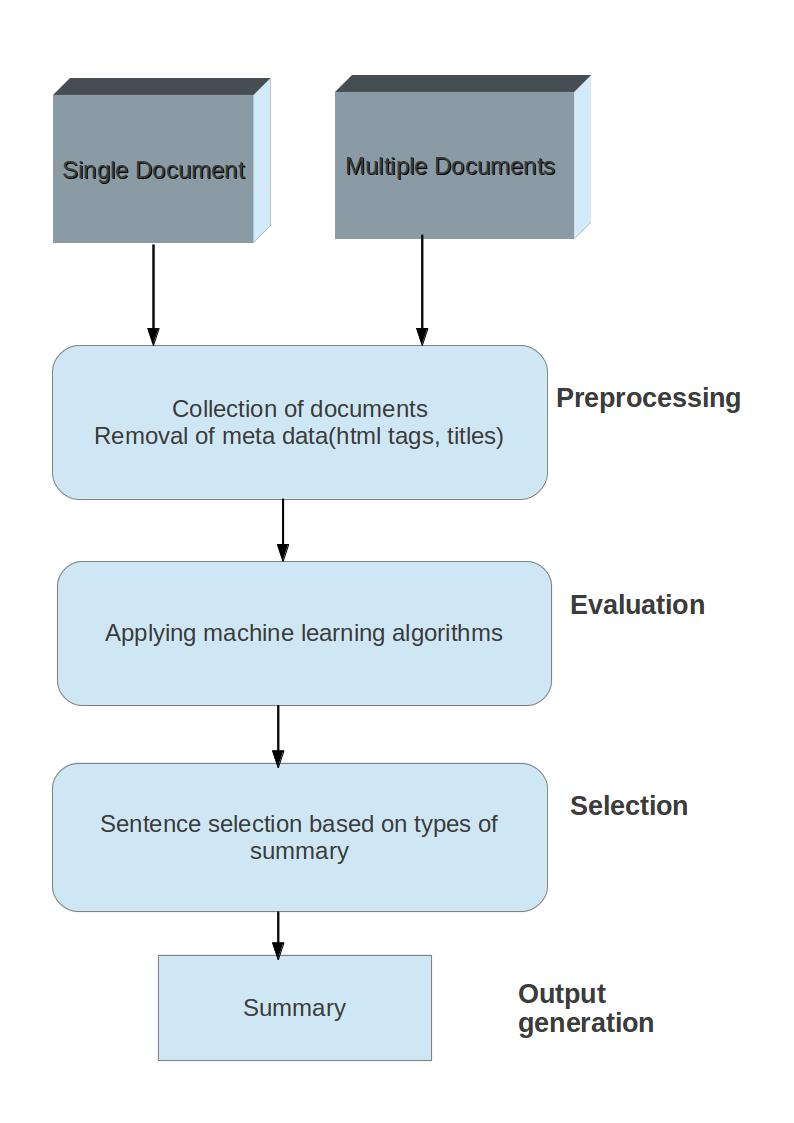
\includegraphics[width=0.5\textwidth]{stages.jpg}
    \caption{Stages of text summarization system.}
\end{figure}
\subsection{Multilingual summarization}
Due to the technological advancements, books and literature from various languages around the world have been digitized. Even though
the literature is available in digital libraries to audiences across the globe, accessiblity to those documents is limited.
End users would like to get some information about a foreign book before getting it translated into language known to them.
Multilingual MDS is very useful in these type of situations. Multilingual summarization will take a very similar approach to 
normal MDS when extracting summaries and then adding a few additional steps in the preprocessing stage. The additional steps in the preprocessing
stage involve language/encoding detection, lemmatization, stemming, indexing. We will discuss each of these steps further in 
the section on the design and implementation of summarization methods for Hindi documents.


\section{Related Work}
Since the early 1960s, several methods have been proposed by researchers. The initial works primarily focused on extracting
sentences based on prominent terms, sentence lengths, random selection. The most prominent study was 
conducted by H.P. Luhn using term frequencies and word collections from \textit{The Automatic Creation of Literature Abstracts}~\cite{Luhn:1958}.
The research aimed to obtain generic abstracts for several research papers. This approach was able to handle only single
documents with less than 4000 words total. Another important approach in the early stages was proposed by Edmundson~\cite{Edmundson:1969}
using term frequencies and emphasizing the location of the sentences. Sentences at the beginning and end were given
priority over other sentences. In the recent past, several methods have been proposed based on statistical, graph based and
machine learning approaches.
\subsection{Statistical approach}
In the statistical approach, features in sentences are selected based on concepts like co-occurrences of words and classification.
Summarist~\cite{Hovy99} is a system proposed by Hovy and Lin, which is based on a statistical approach for sentence extraction from single documents. 
It defines optimal position policy by selecting words based on a certain distribution and extracts sentences containing
the filtered words. Nomoto~\cite{Nomoto05} proposed using bayesian classification in text summarization, the system was
defined for SDS in Japanese and, in some cases, evaluated better than other systems. There are some other 
papers~\cite{Daume:2006} that used lexical chains and bayesian method for sentence extraction. These approaches used supervised
algorithms, which had to be trained in a specific domain to obtain good summary results. This approach was not efficient for
new corpora from a different domain.

\subsection{Graph-based approach}
In the graph based approach each node represents a sentence from the text and nodes are connected to each other using edges.
Nodes are connected to each other only when there are common terms between two nodes and the consine similarity between them
is above certain threshold. From the graph based approach, topic-driven summarization can be done by obtaining a sub-graph which
is similar to the topic. For a generic summary, the most connected node from each sub-graph is selected for the summary.
This approach was used in ranking web pages by Google's PageRank,~\cite{pagerank} which serves to index and search web pages.
Summarization systems like \textit{TextRank~\cite{TextRank}, LexRank~\cite{lexrank}, Hypersum~\cite{Wang:2009}} use this approach for text.
These systems obtain good summaries but get complicated when introduced to MDS.

\subsection{Machine learning approach}
Summarization techniques using machine learning algorithms combined with NLP have increased lately. Machine learning algorithms
like Naive-Bayes, special clustering, classification methods, decision tress, markov models are being used in the implementation
of summaries. Some of their noteworthy approaches includes using the Hidden Markov Models(HMM)~\cite{hmm} and Naive-Bayes~\cite{naive-bayes}.
These approaches work well with SDS but do not scale well to multi-documents. Learning algorithms like Latent Semantic Analysis(LSA)
and Latent Dirichlet Allocation(LDA)~\cite{lda-lsa} work well with single documents and have been highly recommended by TAC.
LSA will be explained in detail in the next section.
\subsubsection{LSA in summarization}
Latent Semantic analysis is the most prominent algebric learning algorithm used for Information Retrieval(IR) from textual data. LSA, is widely used
in various applications for the dimension reduction of large multi-dimensional data. Singular Value Decomposition(SVD) is the most
commonly used learning algorithm for information retrieval. It is known by different names in different fields, Principal Component
Analysis(PCA) in signal processing, KL Transform in image processing, LSA in textual processing. LSA works very well in
single document summarization~\cite{Steinberger:2009} and has been evaluated highly by TAC. Because LSA is an unsupervised
learning algorithm it can be used across different domains without any corpora training. LSA obtains summaries in three
stages: \textit{Input matrix, singular value decomposition, and sentence selection}. \newline
Input matrix(A): In this stage the original documents are transformed into a matrix which can be processed in SVD step. Transformation
of a document involves many NLP methods like segmentation, stemming, word filtering, sentence removal. Values in the matrix signify
the importance of terms in a document and are calculated using different weighting metrics. The selection of a weighting metric can affect
the end results. Some of the weighting metrics are term frequency(tf), term frequency-inverse document frequency (tf-idf), 
log entropy and binary representation(0, 1). All these steps are explained in design implementation section.\newline
\begin{figure}[ht!]
  \centering
    \includegraphics[width=0.5\textwidth]{svd.jpg}
    \caption{Singular value decomposition.}
\end{figure}

Singular value decomposition, is a statistical tool for dimension reduction and feature selection. SVD factorizes a given input
matrix into three matrices as shown above (Figure 2).\newline

\begin{equation}
 A  = U \Sigma V^T
\end{equation}
\begin{center}
\begin{tabular}{ll}
A:&Input matrix (m*n)\\
U:& Orthogonal left singular matrix (m*k)\\
$\Sigma$:& Scalar values matrix (k*k)\\
$V^T$:& Orthogonal right singular matrix (k*n)\\
\end{tabular}
\end{center}

The input matrix comprises values which are defined by the weighting metric and the number of times a term has appeared in a sentence.
Term frequency per sentence is usually zero or one if input matrix is a big (m x n) matrix with rows
defined by terms and columns by sentences. After the decomposition of the input matrix, we obtain two orthogonal matrices and
one diagonal matrix. SVD is similar to eigen value decomposition, the only difference being SVD can be applied on rectangular 
matrices, but eigen decomposition is strictly used for square matrices.\newline
The values of each matrix can be obtained from the original input matrix.
\begin{itemize}
\item left singular matrix U is comprised of eigen vectors of $A A^T$
\item diagonal matrix $\Sigma$ is comprised of eigen values from $\sqrt{(A A^T) (A^T A)}$
\item right singular matrix $V^T$ is comprised of eigen vectors of $A^T A$
\end{itemize}
The left matrix U provides a relationship between terms and features. Any information related to terms can be extracted from matrix U.
For information related to sentences and features, right matrix $V^T$ can be used. Reduction of dimension is based on number
of features (k) required. SVD works well in dimension reduction and text summarization, but it has a few disadvantages. SVD is a time consuming process
and it has to be reworked every time there are any changes to the original matrix. In addition, it cannot identify homonyms and words with
different meanings. These issues can cause problems for large text analysis and summarization.\newline
In the sentence selection stage, different algorithms can be used on the right singular matrix($V^T$) obtained from the SVD on input
matrix. $V^T$ is comprised of \textit{features x sentences}, where \textit{features} are represented by values in rows and \textit{sentences}
by columns. In his paper~\cite{Gong-Liu},  Gong discusses usage of sentences with highest value for each feature. Steinberger \etal
~\cite{Steinberger:2009} used top k sentences with sum of feature values. Clustering algorithms can be used to select sentences
similar to centroids.


\section{Hypothesis}
This project will focus on obtaining well-defined summaries for large data sets of multi-documents through LSA. The use of
different NLP algorithms to improve summaries is examined. Scalability of this approach in a parallel framework will be
analyzed. Results obtained from usage of different weighting metrics (tf-idf, tf, log-entropy) will be compared. Results obtained from different sentence selection approaches will be compared.
This project will take a holistic approach towards LSA summarization techniques, resolve shortcomings of scalability 
, evaluate of previous works that used LSA. This project will attempt to summarize data sets in Hindi and English.
Evaluation of summaries will be done using ROUGE metrics, and the system will be evaluated and compared to current techniques.


\section{Solution}
\subsection{Design}
The general design for text summarization implementation will include several components. The key components in the three 
stages (\textit{input matrix, SVD, sentence selection}) are explained below. A generic design involving components in each
stage can be seen in Figure 3. NLP frameworks used in each of the stages are explained below.
\subsubsection{Datasets}
In this project, experiments will be conducted on both English and Hindi data sets. AQUAINT and AQUAINT2~\cite{aquaint} corpus collections
will be used for english summarization. As there are no data sets available in hindi, we will use documents written in hindi as
our data set.
\subsubsection{Computation resources}
For better performance and speed, experiments will be run on Amazon EC2 AMIs. All the experiments will be conducted on Linux
OS, and host will have minimum memory of 6GB. Performance and speed of algorithms on multiple EC2 instances will be studied.
\begin{figure}[ht!]
  \centering
    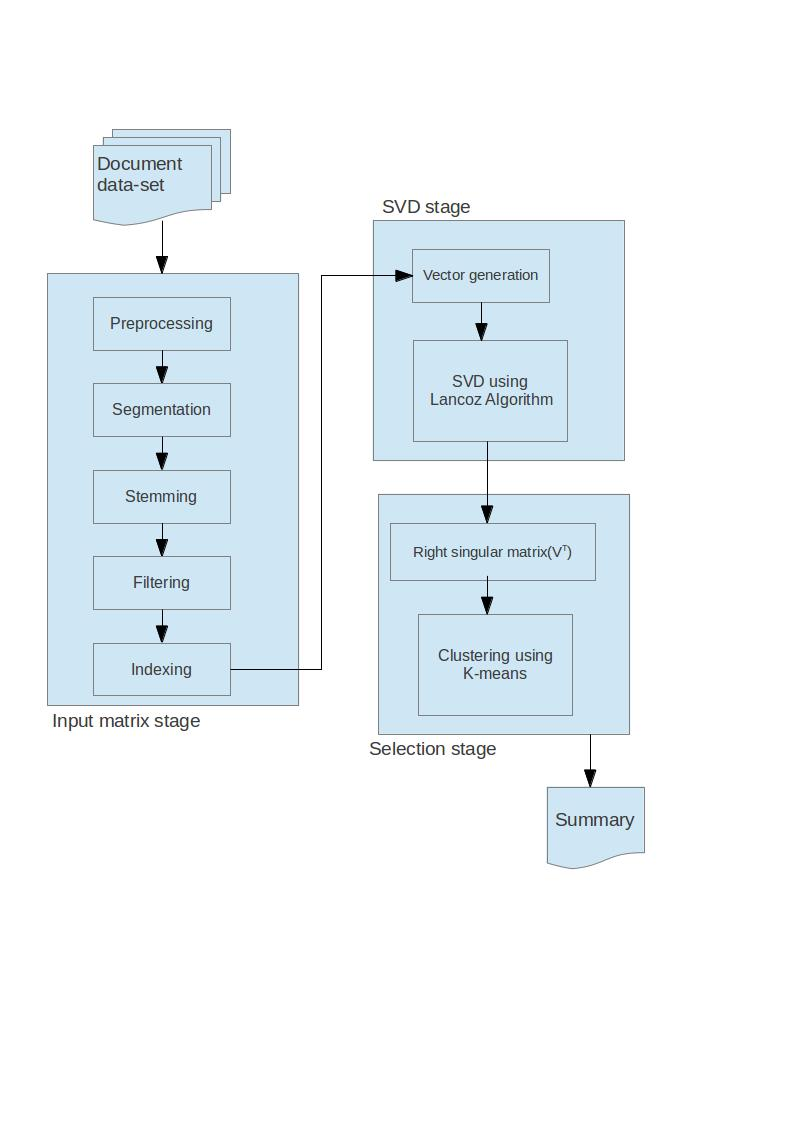
\includegraphics[width=0.5\textwidth]{design.jpg}
    \caption{System Design.}
\end{figure}
\subsection{Implementation}
The project will be implemented using Java programming language and evaluated using Perl. Lucene and Mahout are Java
 APIs which will be used for several information extraction algoritms (as described in 5.2.1 and 5.2.2). Other open-source java-based APIs like Tika and Open-NLP
 will be used. For evaluation purposes, ROUGE tool-kit will be used.
\subsubsection{Lucene}
Lucene API supports indexing of text in different formats like .html, .txt, several other document formats. PDF documents also can be
indexed with the support of an external API named Tika~\cite{tika}. Lucene API will be used for all the components in the input matrix stage.
Preprocessing will involve removal of html tags, extraction of text from different formats, and conversion of text from different
languages to unicode. Segmentation of content can be done based on groups of phrases, collection of sentences or single sentences. 
It is known that usage of single sentences provides better results. In this project, we will segment text based on senteces.
Using different segmentation methods will affect the nature of matrix, i.e., it will be sparse or dense. Word grouping is done through stemming where words like ``running,'' ``runner,'' ``run'' are considered as ``run''.
Using lucene API, words and sentences are filtered to match pre-defined criteria.

In indexing step, lucene will be used to index terms in each sentence. Lucene stores meta-data from documents in the form of 
key-value pairs, where key is the term and value is number of times it occurs in the sentence. Information related to sentences is
provided in the index.
\subsubsection{Mahout}
Mahout API provides access to machine learning algorithms, which can be run on hadoop framework to parallelize the jobs.
Indexed terms from each sentence are converted to vectors based on a selected weighting metric (\textit{tf-idf, tf, log-entropy}).
In the SVD stage, lancoz algorithm will be used on the term vectors to obtain $V^T$. In the sentence selection, k-means algorithm
is implemented using mahout API to obtain k clusters. Sentences from the k clusters are picked based on the similarity of each sentence to
its centroid.
\subsubsection{Parallelization strategy}
Right and left singular eigen vectors can be obtained from  matrix A by matrix multiplication $A A^T$, $A^T A$ respectively.
If A is not a square matrix, a few optimizations have to be done to make it a square matrix. Matrix multiplication can be parallelized
very effectively as a specific row does not have dependency over other rows or columns. Map-reduce framework will be used to
parallelize the indexing of documents and the lancoz algorithm.
\subsection{Evaluation}
Summary evaluation is an important step in understanding how the system has performed. In this project, we will be comparing 
the results from our system against summaries from tools like lexrank and textrank. The summary obtained will be analyzed using 
ROUGE tool-kit~\cite{rouge}. ROUGE n-gram scores and ROUGE LCS scores for different NLP approaches will be compared.


\section{Roadmap}

\subsection{Deliverables}
\begin{itemize}
\item A project report consisting of design, implementation details, experiments, results
and evaluation of summaries
\item The source code
\item Javadoc
\item A manual for using the text summarization system
\item A presentation on project defense
\end{itemize}
\subsection{Schedule}
\begin{itemize}
\item Completion of implementation - second week of July,
\item Completion of experiments on local corpora - third week of July,
\item Formal project proposal submission - fourth week of July,
\item Evaluation and comparisons of summaries - third week of August,
\item Project defense - first week of September.
\end{itemize}

%%%%%%%%%%%%%%%%%%%%%%%%%%%%%%%%%%%%%%%%%%%%%%%%%%%%%%%%%%%%%%%%%%%%%%%%%%%%%%%

%%%%%%%%%%%%%%%%%%%%%%%%%%%%%%%%%%%%%%%%%%%%%%%%%%%%%%%%%%%%%%%%%%%%%%%%%%%%%%%
\bibliographystyle{plain}
% Single space the bibliography to save space.
\singlespacing
\bibliography{Bhargav}
%%%%%%%%%%%%%%%%%%%%%%%%%%%%%%%%%%%%%%%%%%%%%%%%%%%%%%%%%%%%%%%%%%%%%%%%%%%%%%%


\end{document}
